\documentclass{article}
\usepackage{ctex}
\usepackage{hyperref}
\usepackage{geometry}
\usepackage{amsmath}
\usepackage{caption}
\RequirePackage{longtable,multirow,array}
\RequirePackage{booktabs}
\usepackage{booktabs}
\usepackage{multicol}
\usepackage{longtable}
\usepackage{booktabs}
\usepackage{algorithm}
\usepackage{algpseudocode}
\usepackage[style=ieee,sorting=nyt]{biblatex}
\assignrefcontextentries[]{*}
\addbibresource{References.bib}
\geometry{left=1in, right=1in, top=1in, bottom=1in}
\hypersetup{hidelinks}
\hypersetup{bookmarksnumbered=true,
	bookmarksopen=true,
	colorlinks=true,
	linkcolor=black,
	citecolor=blue,
	urlcolor=black}
\usepackage{tikz}
\usepackage{pgfplotstable}
\usepackage{pgfplots}
\pgfplotsset{compat=1.18}
\captionsetup{justification=centering}
\captionsetup[figure]{name={Fig.},labelsep=space,labelfont=bf}
\captionsetup[table]{name={Table},labelsep=space,labelfont=bf}
\CTEXoptions[today=old, contentsname=Contents]
\newcommand{\authyear}[1]{\citeauthor{#1} (\citeyear{#1})}
\setmainfont{Arial}

\newcommand{\toB}[1]{\color{blue}#1\color{black}}

\begin{document}
	\title{\vspace{-2.25cm} Multimodal Abnormity-Aware Model\\for Ocular Disease Diagnosis}
	\author{Siqi Pan}
	\date{}
	\maketitle
	
	\section*{Abstract}
	
	TEXT: abstract
	
	\section{Background}
	
	TEXT: Edit background
	
	Ocular diseases can be diagnosed through various methods, including using optical coherence tomography (OCT) and color fundus images. Ophthalmologists usually identify ocular abnormalities to deduce the disease. Traditionally, the diagnosis primarily depends on the professional experience and knowledge of the ophthalmologists, which may result in high misdiagnosis rate and under-utilization of medical data. With the widespread application of artificial intelligence (AI), deep learning (DL) has made great contributions in providing support to patients in remote areas by sharing expert knowledge \autocite{Ichhpujani_Thakur_2021}. By leveraging DL, researchers have developed auxiliary diagnosis programs to help ophthalmologists in the process. Many studies use convolutional neural network (CNN) to analyze ocular images. Some commonly used CNNs are VGG, ResNet, and Inception \autocite{daich2023artificial}. And for segmenting images and finding abnormalities, U-net is widely used \autocite{Ronneberger_Fischer_Brox_2015}. In training CNNs, most studies use transferred learning, which consists of three steps: learning, fine-tuning, and validation.
	
	Some studies directly predict the disease from OCT images.
	\authyear{li2019deep} used ResNet to analyze OCT images and distinguish between choroidal neovascularization (CNV), diabetic macular edema (DME), drusen, and normal eyes. In addition, they performed occlusion testing to find out the regions that are the most important in diagnosis \autocite{li2019deep}. 
	\authyear{yoo2021feasibility} used generative adversarial network (GAN) and Inception-v3 together with a few-shot dataset to investigate the feasibility of improving OCT diagnosis of rare ocular diseases \autocite{yoo2021feasibility}. They cleverly handled the issues of training image shortage and data imbalance by creating ocular disease OCT images from healthy OCT images. \authyear{Kermany2018} conducts medical diagnosis and identifies treatable diseases by image-based deep learning. They also provided a widely used database including more than one hundred thousand OCT labeled images for 3 diseases \autocite{Kermany2018}.
	
	Some other studies can identify ocular abnormalities from annotated OCT images.
	\authyear{camino2018deep} used DL to identify the region of preserved photoreceptors on \textit{en face} OCT in choroideremia and retinitis pigmentosa (RP) \autocite{camino2018deep}. 
	\authyear{srinivasan2014fully} detected DME and dry age-related macular degeneration (dry AMD) from OCT images by flattening the image and using support vector machine (SVM) to extract the thickness information of the retinal layers \autocite{srinivasan2014fully}. 
	\authyear{leandro2023oct} implemented VGG to identify up to 8 kinds of key abnormalities and hence detect multiple diseases by using central fovea cross-section OCT \autocite{leandro2023oct}. \authyear{Fang_Wang2019} developed a novel lesion-aware CNN, called LACNN, to simulate the ophthalmologists' diagnosis that focuses on ocular abnormalities. The LACNN is a U-net-like CNN which incorporates VGG16 as the baseline, and the result is impressive \autocite{Fang_Wang2019}.
	
	Other studies use fundus images to predict ocular diseases.
	\authyear{masumoto2019accuracy} trained deep CNN with ultrawide-field fundus images to make the CNN capable of diagnosing RP \autocite{masumoto2019accuracy}. 
	\authyear{chen2021artificial} uses color fundus photographs and multiple types of CNN (Inception V3, Inception Resnet V2, and Xception) to develop a method of early detection of RP \autocite{chen2021artificial}. 
	\authyear{li2022development} uses CNN to detect up to 12 fundus diseases based on colour fundus photography \autocite{li2022development}. \authyear{Son2023} presented a novel architectural and algorithmic design to comprehensively identify 15 abnormalities and diagnose 8 major ocular diseases from macula-centered fundus images. They defined a notion of counterfactual attribution ratio (CAR) to interpret the system's diagnostic reason and disclose the relationship between abnormalities and diseases \autocite{Son2023}.
	
	In recent years, more and more DL systems began to use multi-modal information to predict ocular diseases. For automated detection system, retrieving features from both OCT images and fundus images can effectively keep the diagnosis away from bias and incompleteness. It is not always necessary to yield a better automated diagnosis result, but it does help ophthalmologist to make more accurate and holistic clinical decisions. For instance, \authyear{liu2023prediction} combined OCT and fundus images to evaluate visual impairment in RP in terms of best-corrected visual acuity(BCVA) \autocite{liu2023prediction}. \authyear{Xu2021} leveraged a bi-modal CNN to diagnose AMD and polypoidal choroidal vasculopathy (PCV), where the architecture uses fundus and OCT images as input for transferred learning CNN and concatenates the retrieved features to classify 3 diseases including dry AMD, wet AMD and PCV \autocite{Xu2021}. And \author{Andrearczyk2018} ingeniously combined medical images and biomedical textual information to discriminate different diseases, which is a novel method for the usage of multi-modal application \autocite{Andrearczyk2018}.
	
	The key technical problem of multi-modal diagnosis is how to fuse the results from multifarious sources. There are three types of fusion, namely early, late, and hybrid fusion. Deciding on the optimal type of fusion is part of the exploratory process in the application of DL methods \autocite{Ichhpujani_Thakur_2021}.
	
	
	
	\section{Overview}
	
	We develop the Multimodal Abnormity-Aware Model (MAAM) to aid ophthalmologists in diagnosing ocular diseases. It considers both OCT and color fundus image inputs. In addition, it simulates the decision-making process of ophthalmologists when they examine patients, i.e., first identifying the abnormities, and then deducing the disease. The model is designed in a way that partly opens up the ``black box'' of DL and presents more interpretable information for the reference of ophthalmologists. 
	
	\begin{figure}[htbp]
		\centering
		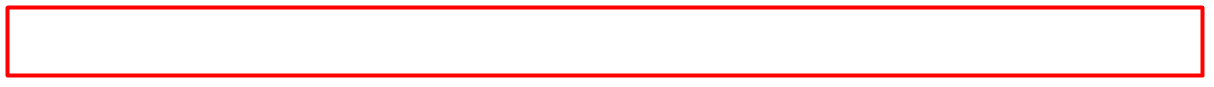
\includegraphics[width=\linewidth]{Figs/Temp.png}
		\caption{Model Overview}
		\vspace{0.3cm}
		\label{fig:3_parts}
	\end{figure}
	
	The structure of the MAAM is shown in Fig.~\ref{fig:3_parts}. It consists of 2 submodels: the Abnormity Models and the Diagnosis Model. We input multiple OCT and fundus images to the Abnormity Models, and output the classification of abnormities as inputs to the Diagnosis Model, which generates disease probabilities as the final result.
	
	\vspace{0.5cm}
	
	The Abnormity Models are classifiers for abnormities, which are symptoms that can be directly observed in the images. The MAAM identifies 11 OCT abnormities and 8 Fundus abnormities, as shown in Fig.~\ref{fig:OCT_abnormities} and Fig.~\ref{fig:fundus_abnormities}. Also refer to ``Appendix'' for more details.
	
	\begin{figure}[htbp]
		\centering
		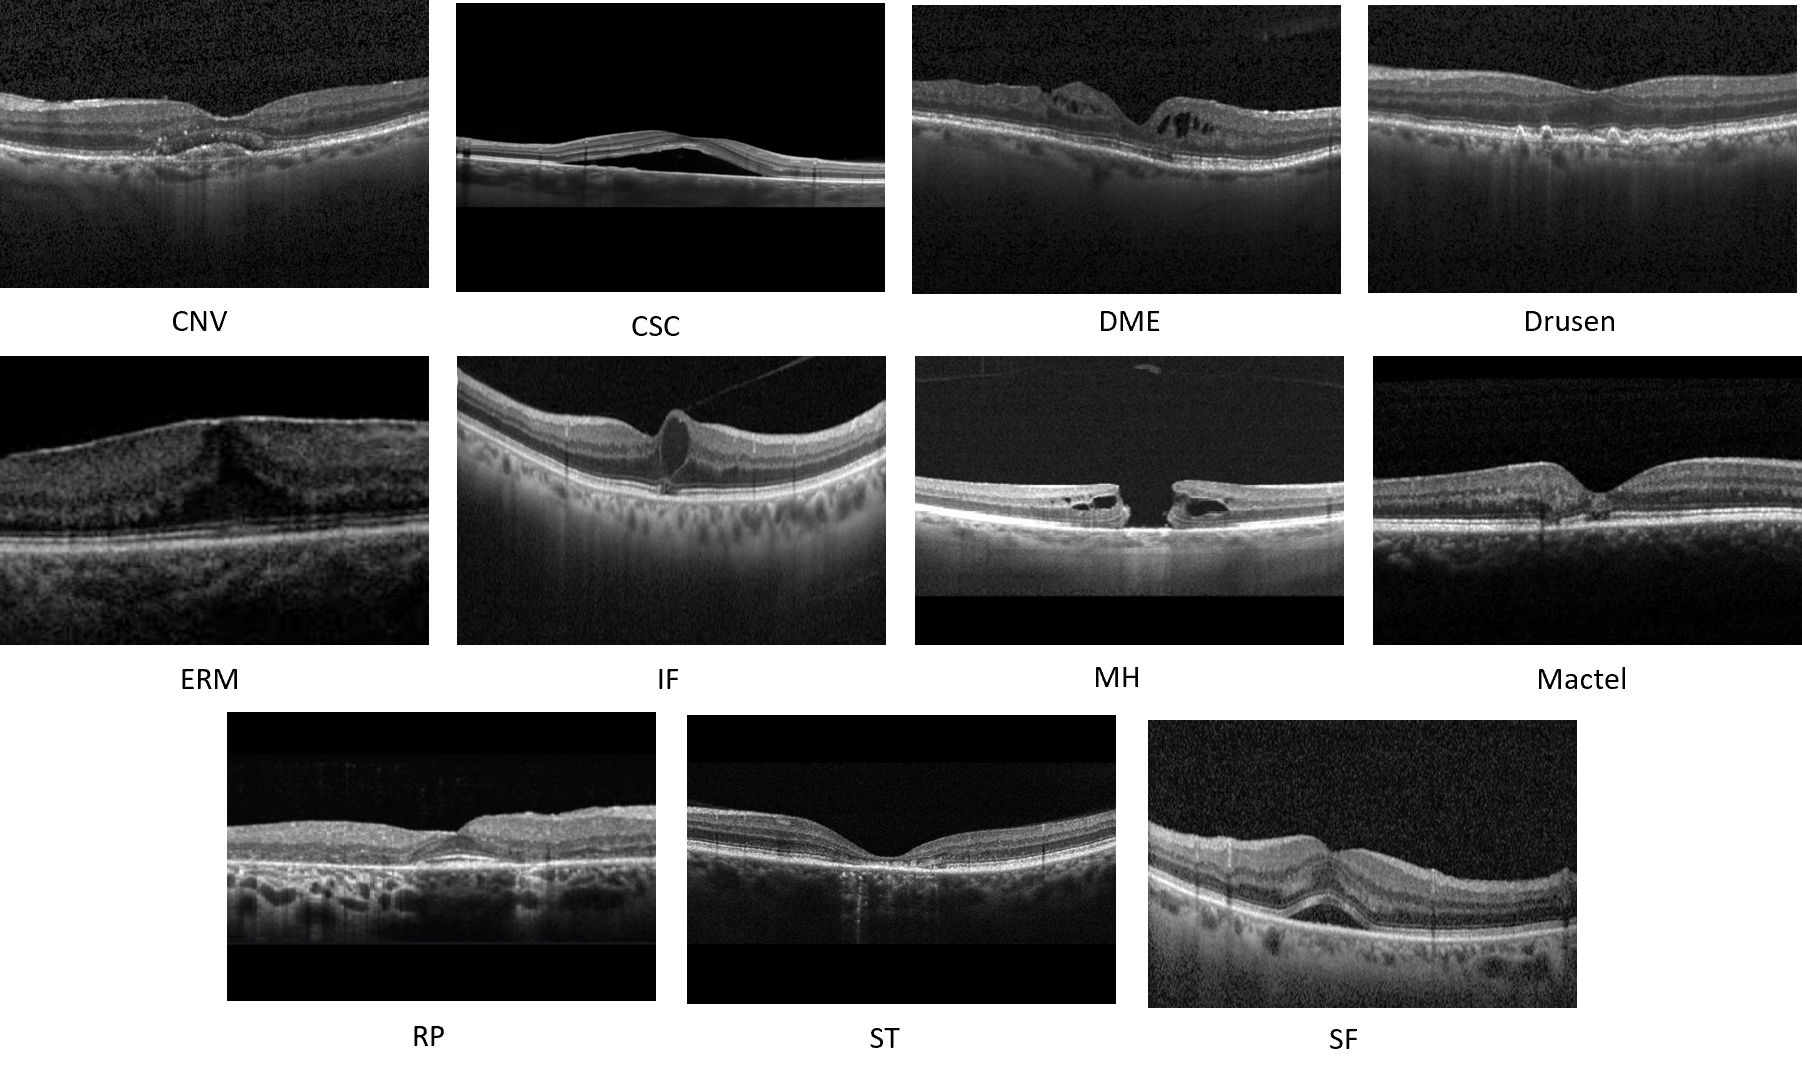
\includegraphics[width=\linewidth]{Figs/OCT_Abnormities.png}
		\caption{OCT Abnormities}
		\vspace{0.3cm}
		\label{fig:OCT_abnormities}
	\end{figure}
	
	\begin{figure}[htbp]
		\centering
		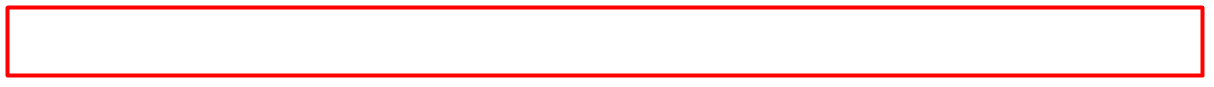
\includegraphics[width=\linewidth]{Figs/Temp.png}
		\caption{Fundus Abnormities}
		\vspace{0.3cm}
		\label{fig:fundus_abnormities}
	\end{figure}
	
	The Abnormity Models also contain 2 submodels: the OCT Model and the Fundus Model, which identify OCT and fundus abnormities, respectively. Both of the submodels leverage CNNs with modified final fully-connected (FC) layers. We compare the performances of 4 commonly used CNNs, ResNet152, ResNet50, ResNet18 and VGG16, and choose the best one for each submodel. The final FC layer in each CNN is modified so that the size of its output vector is equal to the number of OCT or fundus abnormities. In order to normalize the output vector, we perform the softmax operation. After an image is inputted into one of the submodels, the submodel returns a probability vector for all the abnormities.
	
	\vspace{0.5cm}
	
	The Diagnosis Model consists of two stages: Stage D1 and Stage D2. 
	
	\vspace{0.2cm}
	
	In Stage D1, we determine the severity level for each disease from the probability vectors from the Abnormity Models. We use Abnormity-to-Disease Deduction Criteria (shown in Fig.~\ref{fig:criteria}) as ground truth. There are multiple submodels in Stage D1 and each one corresponds to one disease. From the deduction criteria, we determine the number of abnormities for one disease and use the number to define the severity levels. For example, there are totally 5 abnormities that are present in the disease ``Referable DR'': OCT abnormity ``DME'' and Fundus abnormities ``Hemorrhage'', ``Vascular Abnormity'', ``Microaneurysm'', and ``Cotton Wool Patch''. Therefore, taking into account the healthy status, we end up with 6 severity levels for disease ``Referable DR''.

	We use the fused vector as an input for each submodels in Stage D1, and have the vector pass a FC layer with softmax operation to generate severity level probability vectors.
	
	\begin{figure}[htbp]
		\centering
		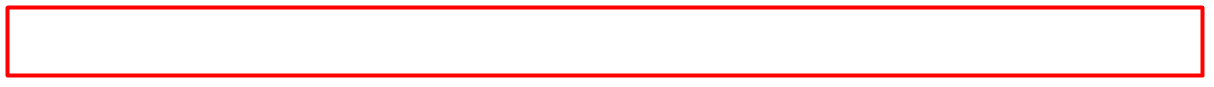
\includegraphics[width=\linewidth]{Figs/Temp.png}
		\caption{Abnormity-to-disease Deduction Criteria}
		\vspace{0.3cm}
		\label{fig:criteria}
	\end{figure}

	\vspace{0.2cm}
	
	In Stage D2, we determine the final disease probability vector. Similarly we use a fused vector from the outputs of submodels in Stage D1, and have the vector pass a FC layer with softmax operation. The result presents potential diseases that can be referenced by ophthalmologists.

	\vspace{0.5cm}
	
	In the MAAM, we leverage the fusion operation to incorporate all the results from different submodels. As shown in Fig.~\ref{fig:fusion}, there are 3 fusion operations in MAAM.
	
	\begin{figure}[htbp]
		\centering
		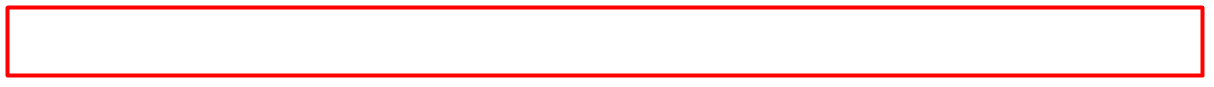
\includegraphics[width=\linewidth]{Figs/Temp.png}
		\caption{Fusion}
		\vspace{0.3cm}
		\label{fig:fusion}
	\end{figure}

	The first fusion occurs at the output of OCT Model or Fundus Model. In real cases, multiple OCT and Fundus images can be used for ocular disease diagnosis. Each image goes through one of the Abnormity Models and generates a probability vector. To use the probability results from all the images, a maximization fusion is implemented for all the vectors so that the fusion yields one OCT abnormity probability vector and one Fundus abnormity probability vector with maximum values.
	
	The second fusion occurs at the interface between Abnormity Model and Stage D1. A concatenation fusion is implemented for OCT abnormity probability vector and Fundus abnormity probability vector. The fused vector works as an input to all the submodels in Stage D1.
	
	The third fusion occurs at the interface between Stage D1 and Stage D2. We concatenation all the severity level vectors to feed the model in Stage D2. The fused vector goes through the FC layer and undergoes a softmax operation to yield the final result.
	
	\section{Abnormity Models}
	
	\subsection{Data Preparation}
	
	\begin{figure}[htbp]
		\centering
		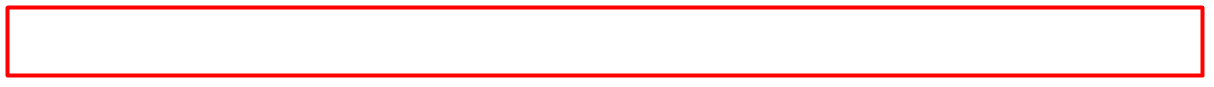
\includegraphics[width=\linewidth]{Figs/Temp.png}
		\caption{Data preparation for abnormity models}
		\vspace{0.3cm}
		\label{fig:A_data_prep}
	\end{figure}
	
	The data preparation process is shown in Fig.~\ref{fig:A_data_prep}. 
	
	First, we acquire data from publicly available online datasets. For abnormities with no data found, we search for images on Google Image. The numbers of images acquired from each data source are shown in Table~\ref{tb:OCT_source} and Table~\ref{tb:Fundus_source}. For the links of the images from Google Image, please refer to ``Appendix''. 
	
	\begin{minipage}[t]{0.4\linewidth}
		{
			\fontsize{9}{12}\selectfont
			{
				\begin{longtable}{cccccc}
					\caption{OCT abnormities}
					\label{tb:OCT_source}\\
					\toprule
					\multirow{2}{*}{Abnormity}&\multicolumn{4}{c}{Source}&\multirow{2}{*}{Total}\\
					&1&2&3&4&\\
					\midrule
					CNV    &2984&/  &/ &/ &2984\\
					CSC    &/   &102&32&/ &134 \\
					DME    &2500&/  &/ &/ &2500\\
					Drusen &2500&/  &/ &/ &2500\\
					ERM    &/   &/  &/ &19&19  \\
					IF     &1097&/  &/ &/ &1097\\
					MH     &/   &99 &31&/ &130 \\
					Mactel &/   &/  &29&/ &29  \\
					Healthy&5000&/  &/ &/ &5000\\
					RP     &/   &102&31&/ &133 \\
					ST     &/   &/  &23&/ &23  \\
					SF     &1083&/  &/ &/ &1083\\
					\bottomrule
				\end{longtable}
				
				\vspace{0.5cm}
				\begin{enumerate}
					\item Normal Disease Database
					\vspace{-0.2cm}
					
					\item OpenICPSR
					\vspace{-0.2cm}
					
					\item Few-shot
					\vspace{-0.2cm}
					
					\item Google Image
					\vspace{-0.2cm}
				\end{enumerate}
				
				\vspace{0.5cm}
			}
		}
	\end{minipage}
	\begin{minipage}[t]{0.6\linewidth}
		{
			\fontsize{9}{12}\selectfont
			{
				\begin{longtable}{cccccccc}
					\caption{Fundus abnormities}
					\label{tb:Fundus_source}\\
					\toprule
					\multirow{2}{*}{Abnormity}&\multicolumn{6}{c}{Source}&\multirow{2}{*}{Total}\\
					&1&2&3&4&5&6&\\
					\midrule
					CWP    &/  &/ &/ &33 &205&/ &238\\
					Drusen &/  &/ &/ &50 &/  &/ &50 \\     
					HE     &20 &/ &/ &75 &284&/ &379\\ 
					HM     &13 &66&/ &105&278&/ &462\\     
					MH     &/  &/ &/ &/  &/  &34&34 \\        
					MA     &55 &/ &/ &1  &219&/ &275\\
					Healthy&100&37&15&/  &/  &/ &152\\      
					RP     &/  &22&/ &/  &/  &44&66 \\         
					VA     &/  &64&/ &14 &/  &/ &78 \\
					
					\bottomrule
				\end{longtable}
				
				\vspace{1cm}
				\begin{enumerate}
					
					\item E-ophtha
					\vspace{-0.2cm}
					
					\item Kaggle1000
					\vspace{-0.2cm}
					
					\item HRF
					\vspace{-0.2cm}
					
					\item STARE
					\vspace{-0.2cm}
					
					\item EyePACS
					\vspace{-0.2cm}
					
					\item Google Image
					\vspace{-0.2cm}
					
				\end{enumerate}
				
				\vspace{0.5cm}
			}
		}
	\end{minipage}
	
	Then, for OCT abnormities with less than 1000 images, we use Cycle-GAN to generate new images. We train a Cycle-GAN network to interconvert healthy and abnormity images, take out the generator that converts healthy to abnormity images, and use it to generate new abnormity images. We manually eliminate generated images that look obviously wrong. The elimination rates are shown in Table~\ref{tb:cycleGAN_number}. We did not use Cycle-GAN to generate fundus images because generated fundus images are too blurry and do not display the desired abnormities.
	
	{
		\fontsize{9}{12}\selectfont
		{
			\begin{longtable}{ccccc}
				\caption{OCT images CycleGAN elimination rates}
				\label{tb:cycleGAN_number}\\
				\toprule
				Abnormity&Original&Generated&Eliminated&Elimination Rate\\
				\midrule
				CSC   &134&3000&1270&42.333\% \\
				ERM   &19 &3000&1069&35.633\% \\
				MH    &130&3000&1189&39.633\% \\
				Mactel&29 &3000&1100&36.667\% \\
				RP    &133&3000&1077&36.900\% \\
				ST    &23 &3000&418 &13.933\% \\
				\bottomrule
			\end{longtable}
		}
	}
	
	We separate the images, including generated images, into training and testing datasets. We implement a set of transformations on the images, including horizontal flips, random brightness changes from -10\% to +10\%, random horizontal and vertical translations between -5\% and +5\%, random scaling between -20\% and +20\%, and random rotations, which are between -10$^\circ$ and +10$^\circ$ for OCT images and between -30$^\circ$ and +30$^\circ$ for fundus images. The rotation is only applied to images in the train dataset. Eventually, we get 5000 train images and 500 test images for each OCT abnormity, and 3000 train images and 300 test images for each fundus abnormity.
	
	\subsection{Training}
	
	We 
	
	TEXT: intro to five-fold train/valid (reason for using this?)
	TEXT: crossentropyloss, ADAM optimizer with LR 1e-3, batchSize 16, number of epochs...
	conda, PyTorch;
	desktop computer with Intel$^®$ Xeon$^®$ Platinum 8352V Processor, 256G of RAM and 2 NVIDIA GPU (GeForce RTX 4090) with 48 VRAM
	
	\begin{figure}[htbp]
		\centering
		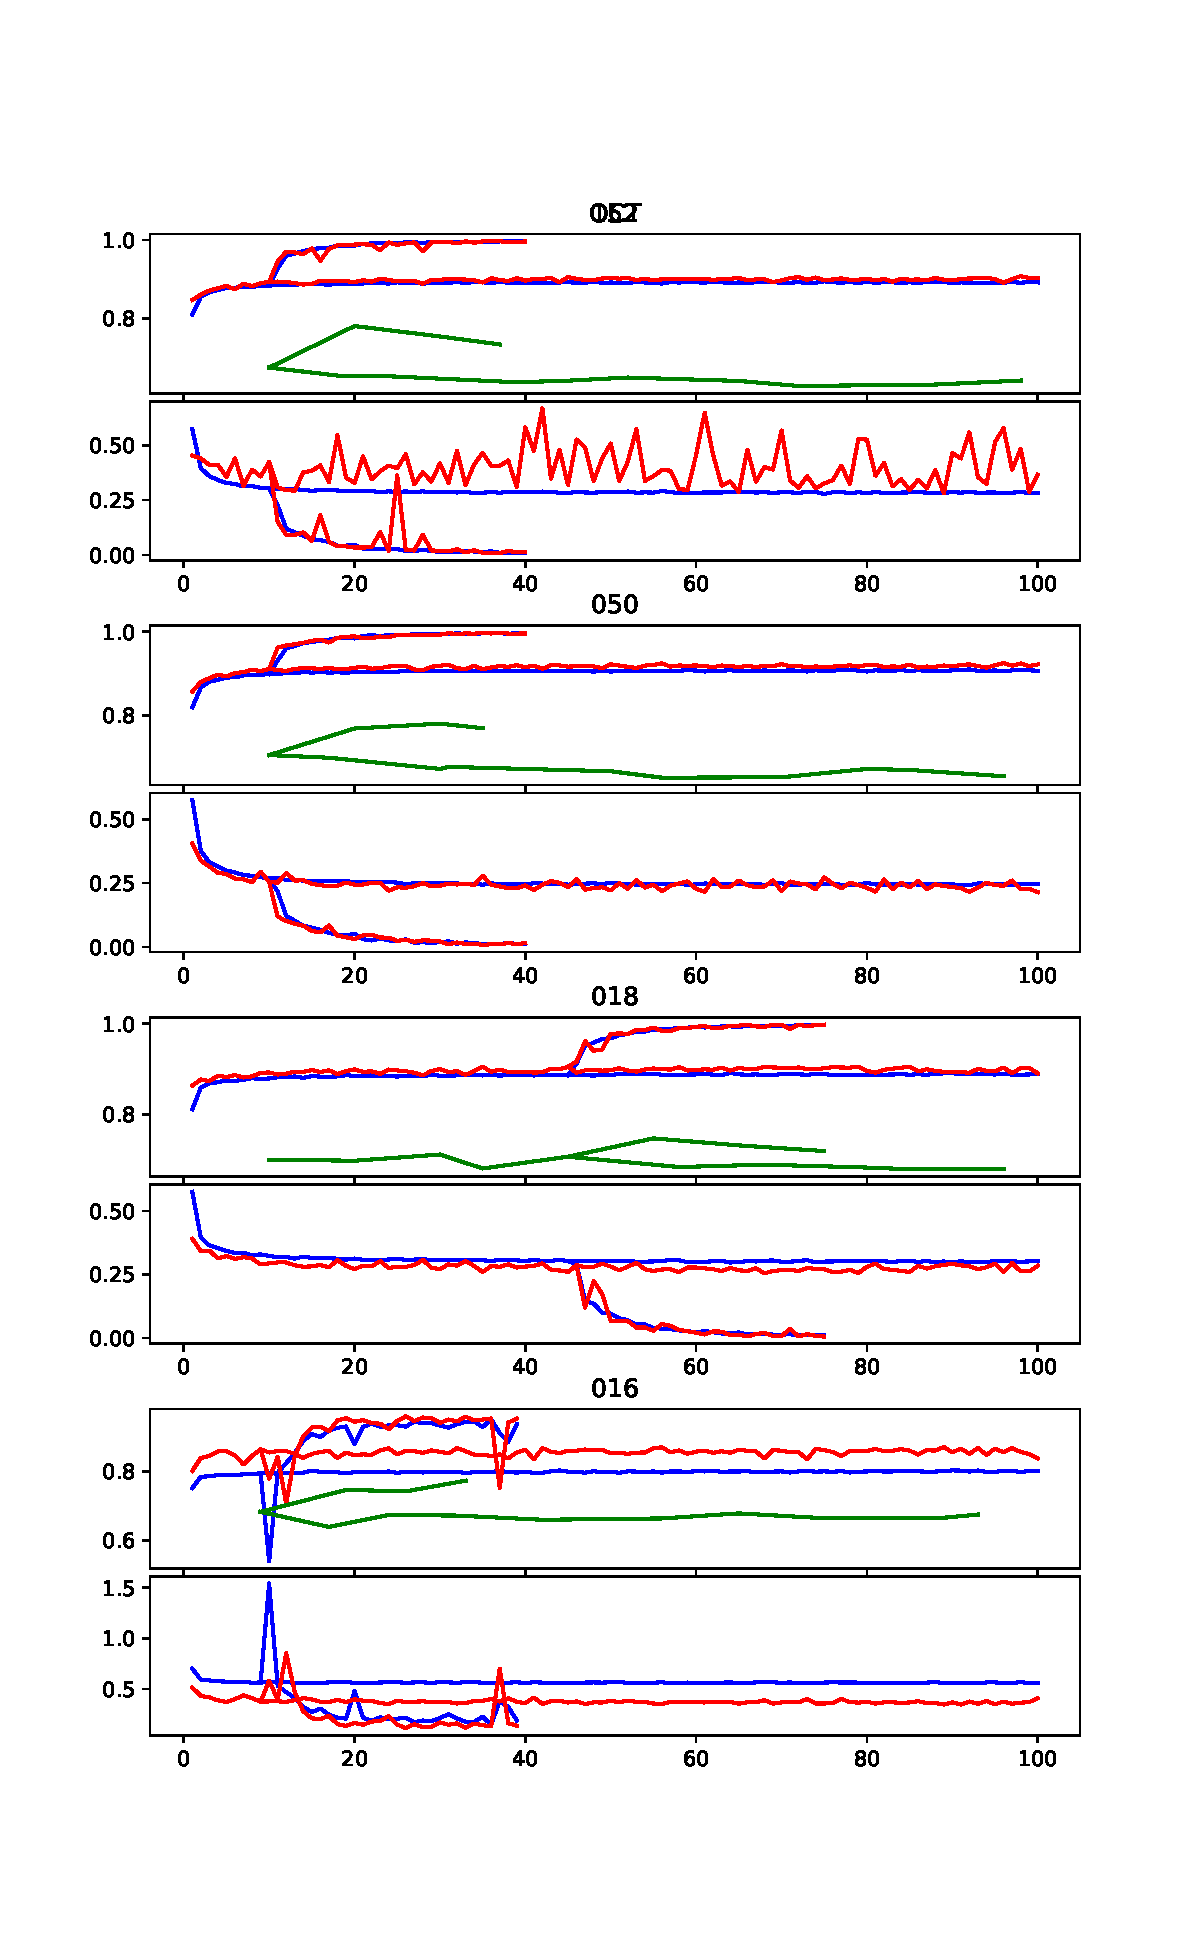
\includegraphics[width=\linewidth]{Figs/abnormity_OCT_loss_and_acc.pdf}
		\caption{AO train}
		\vspace{0.3cm}
		\label{fig:AO_train}
	\end{figure}
	
	\begin{figure}[htbp]
		\centering
		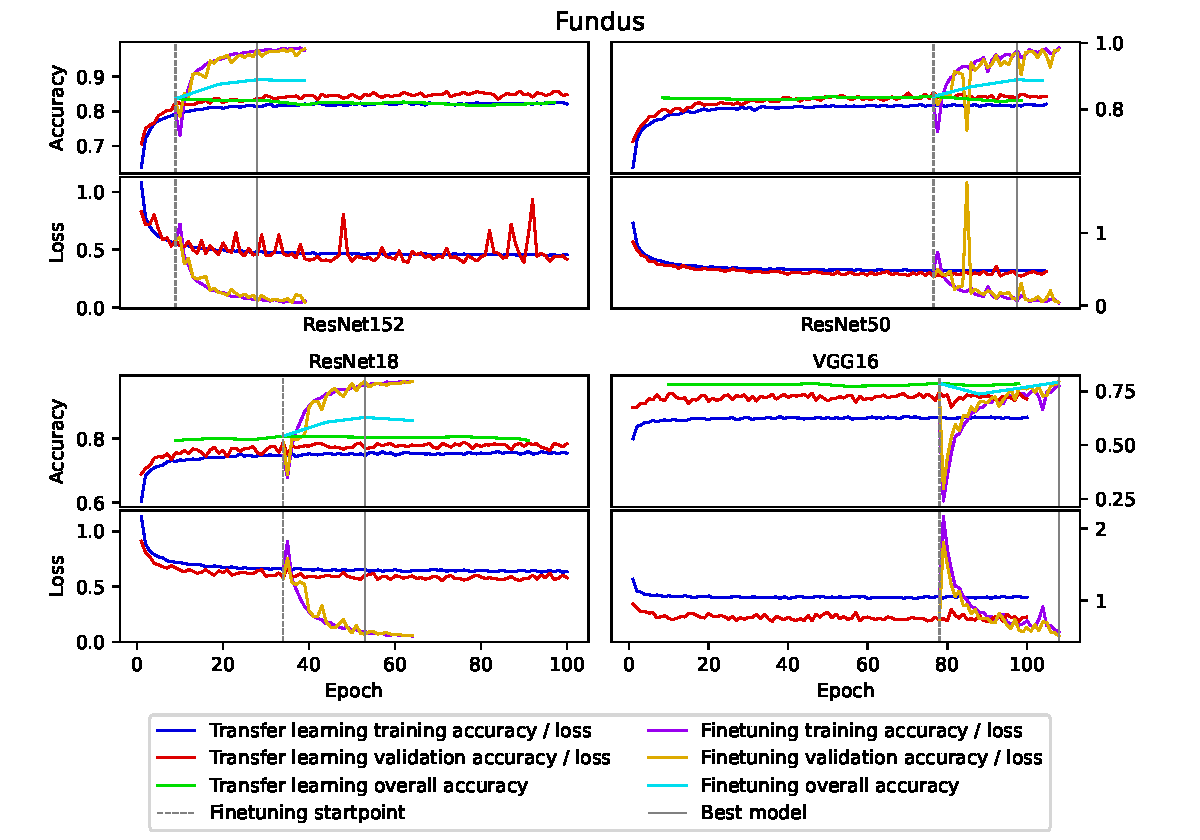
\includegraphics[width=\linewidth]{Figs/abnormity_Fundus_loss_and_acc.pdf}
		\caption{AF train}
		\vspace{0.3cm}
		\label{fig:AF_train}
	\end{figure}
	
	Graph bar chart for comparison? 
	
	TEXT: comments
	
	\subsection{Results}
	
	TEXT: accuracy; explain top-probs method
	
	
	
	\begin{table}[htbp]
		\centering
		\caption{OCT Test}
		\label{tb:OCT_test}
		\pgfplotstabletypeset[
		multicolumn names,
		col sep=comma,
		columns = {Abnormity, Precision, Sensitivity, Specificity, FOne, AUC},
		columns/Abnormity/.style={string type, column name=Abnormities},
		columns/Precision/.style={string type, column name=Precision},
		columns/Sensitivity/.style={string type, column name=Sensitivity},
		columns/Specificity/.style={string type, column name=Specificity},
		columns/FOne/.style={string type, column name={F1 Score}},
		columns/AUC/.style={string type, column name=AUC},
		every head row/.style={before row=\toprule, after row=\midrule},
		every last row/.style={ after row=\bottomrule}
		]{Tables/abnormity_o_test.csv}
	\end{table}
	
	\begin{table}[htbp]
		\centering
		\caption{Fundus Test}
		\label{tb:Fundus_test}
		\pgfplotstabletypeset[
		multicolumn names,
		col sep=comma,
		columns = {Abnormity, Precision, Sensitivity, Specificity, FOne, AUC},
		columns/Abnormity/.style={string type, column name=Abnormities},
		columns/Precision/.style={string type, column name=Precision},
		columns/Sensitivity/.style={string type, column name=Sensitivity},
		columns/Specificity/.style={string type, column name=Specificity},
		columns/FOne/.style={string type, column name={F1 Score}},
		columns/AUC/.style={string type, column name=AUC},
		every head row/.style={before row=\toprule, after row=\midrule},
		every last row/.style={after row=\bottomrule}
		]{Tables/abnormity_f_test.csv}
	\end{table}
	
	\begin{figure}[htbp]
		\centering
		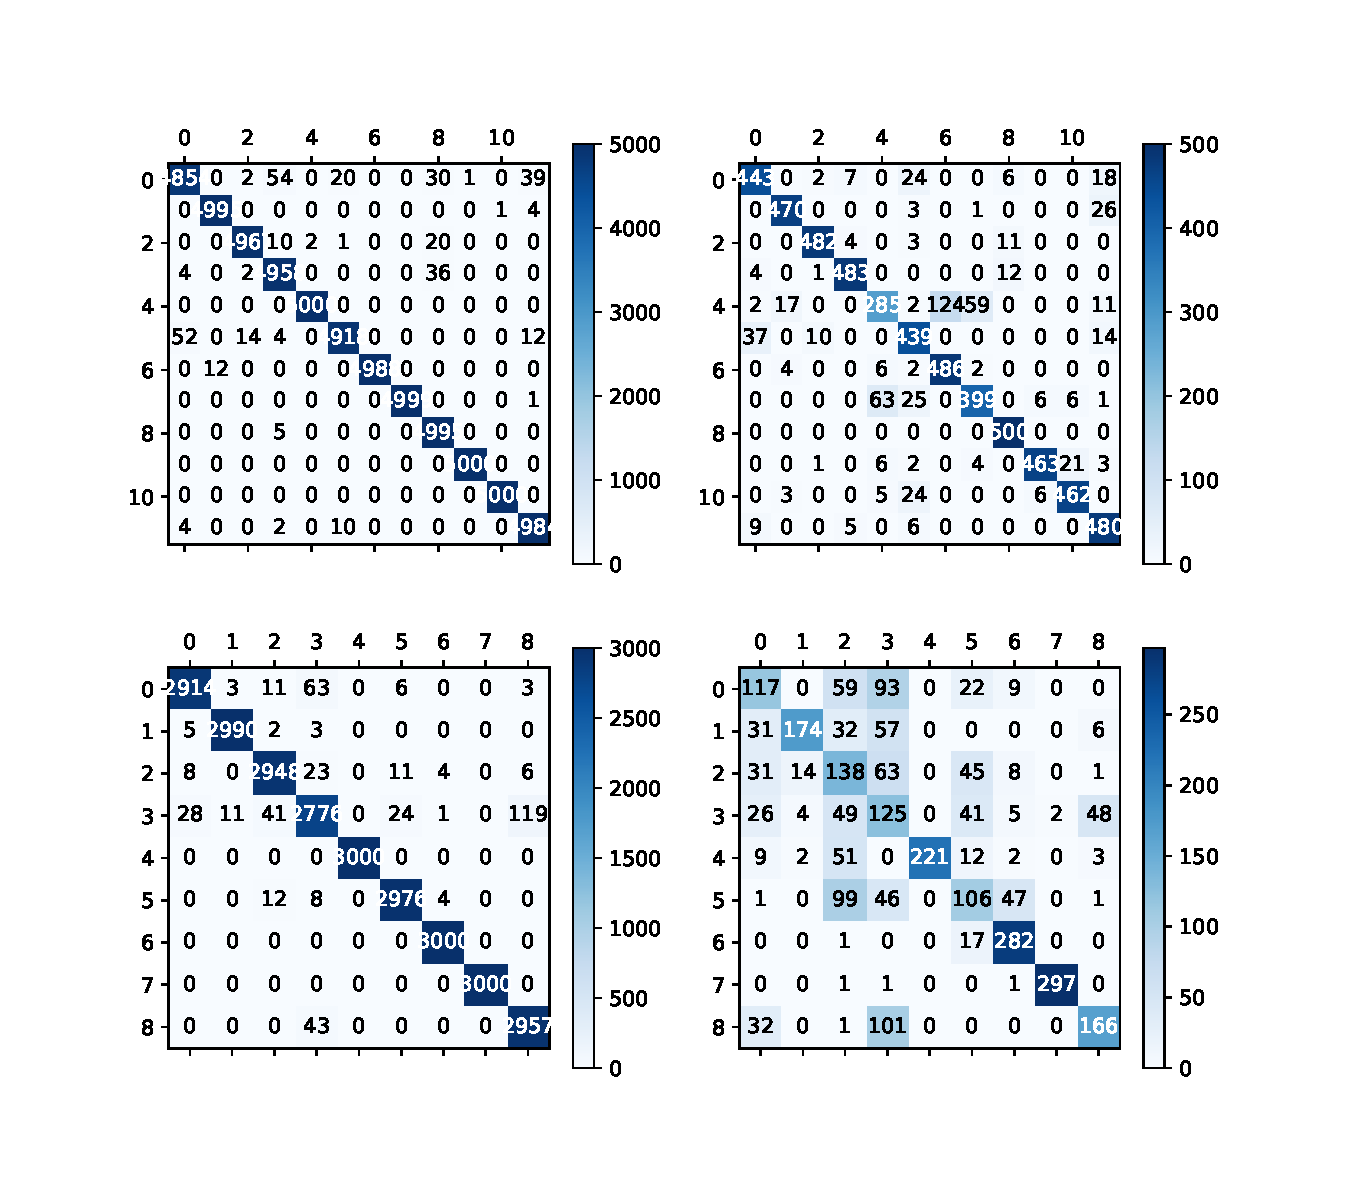
\includegraphics[width=0.8\linewidth]{Figs/abnormity_confusion_matrix.pdf}
		\caption{A Conf Mat}
		\vspace{0.3cm}
		\label{fig:A_conf_mat}
	\end{figure}
	
	TEXT: analyze which abnormities are commonly confused, and the effect on the numerical results
	
	\begin{figure}[htbp]
		\centering
		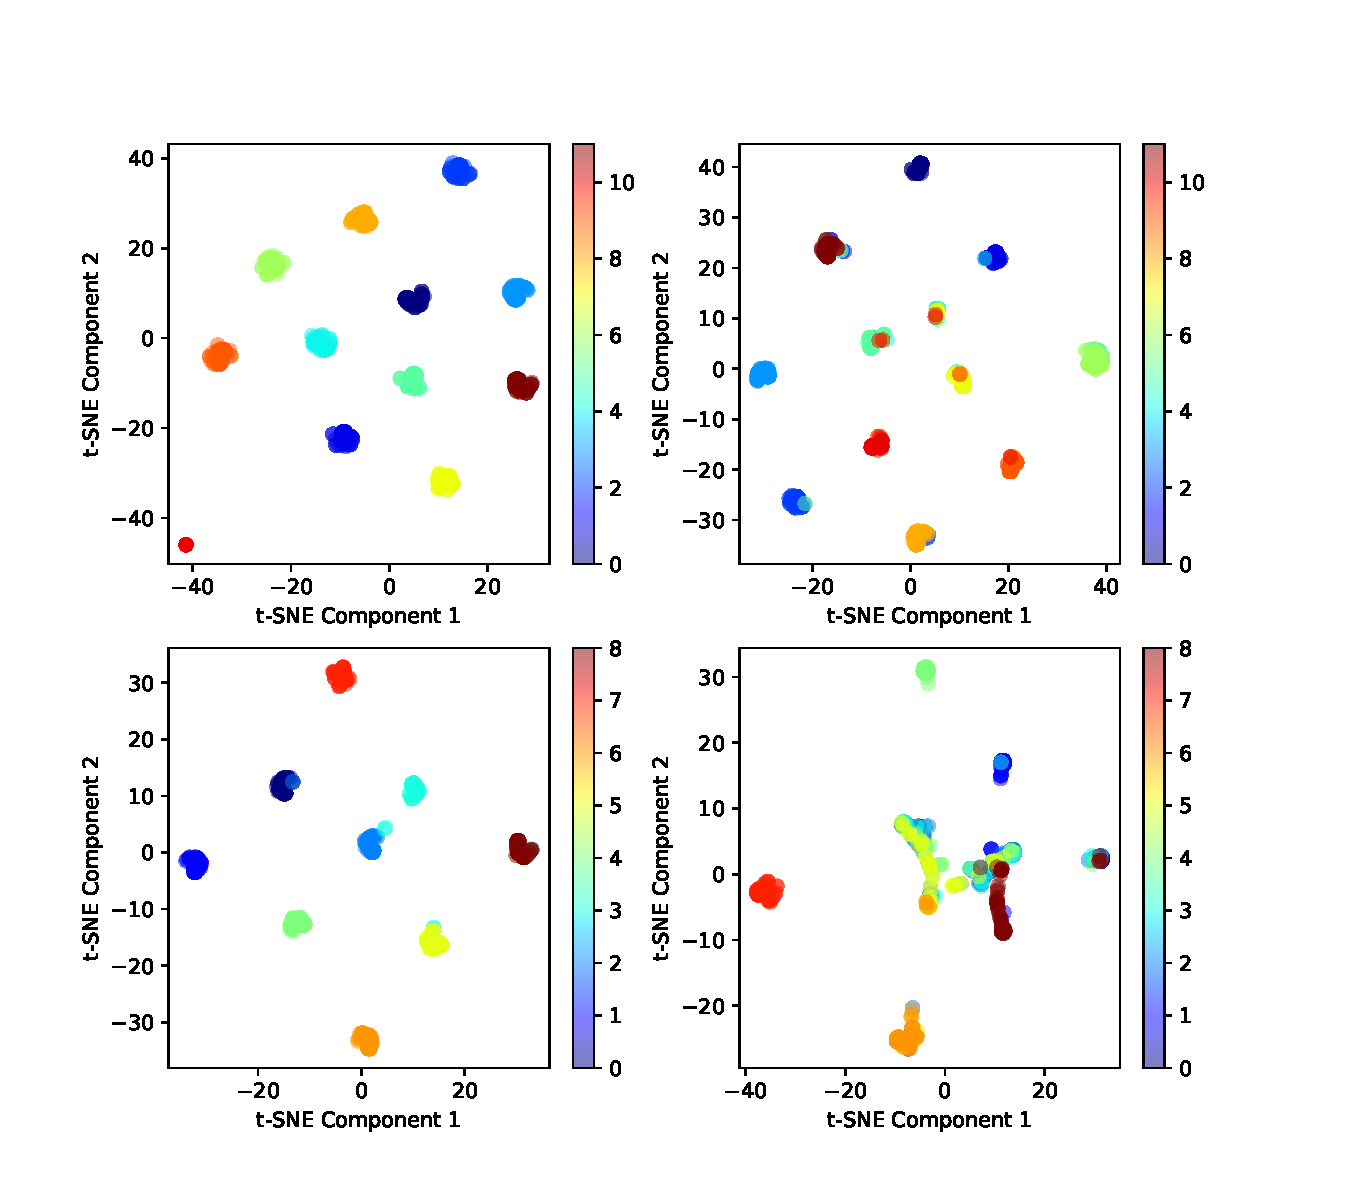
\includegraphics[width=\linewidth]{Figs/abnormity_tSNE.pdf}
		\caption{A ROC}
		\vspace{0.3cm}
		\label{fig:A_tSNE}
	\end{figure}
	
	TEXT: which abnormities are "close"
	
	\begin{figure}[htbp]
		\centering
		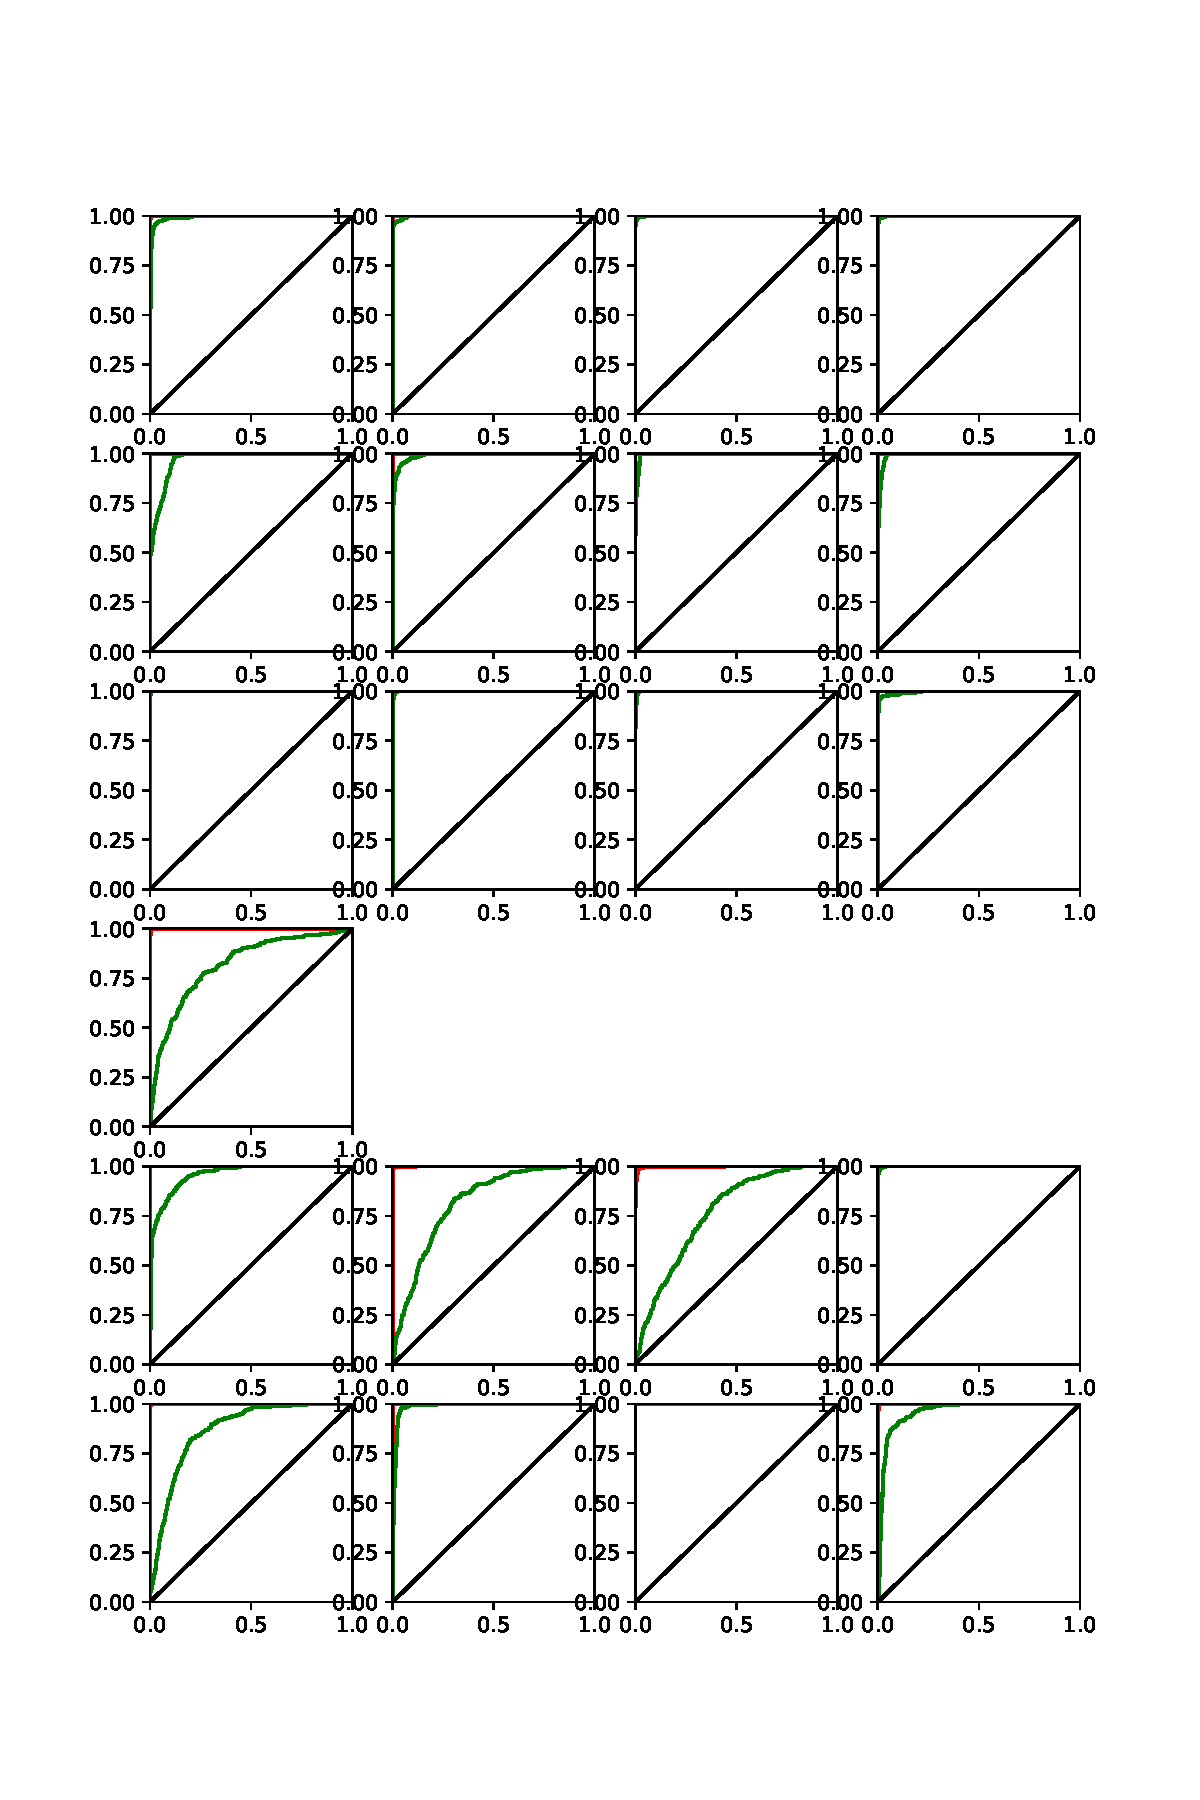
\includegraphics[width=\linewidth]{Figs/abnormity_ROC.pdf}
		\caption{A ROC}
		\vspace{0.3cm}
		\label{fig:A_ROC}
	\end{figure}
	
	TEXT: comparison to other studies
	
	\begin{figure}[htbp]
		\centering
		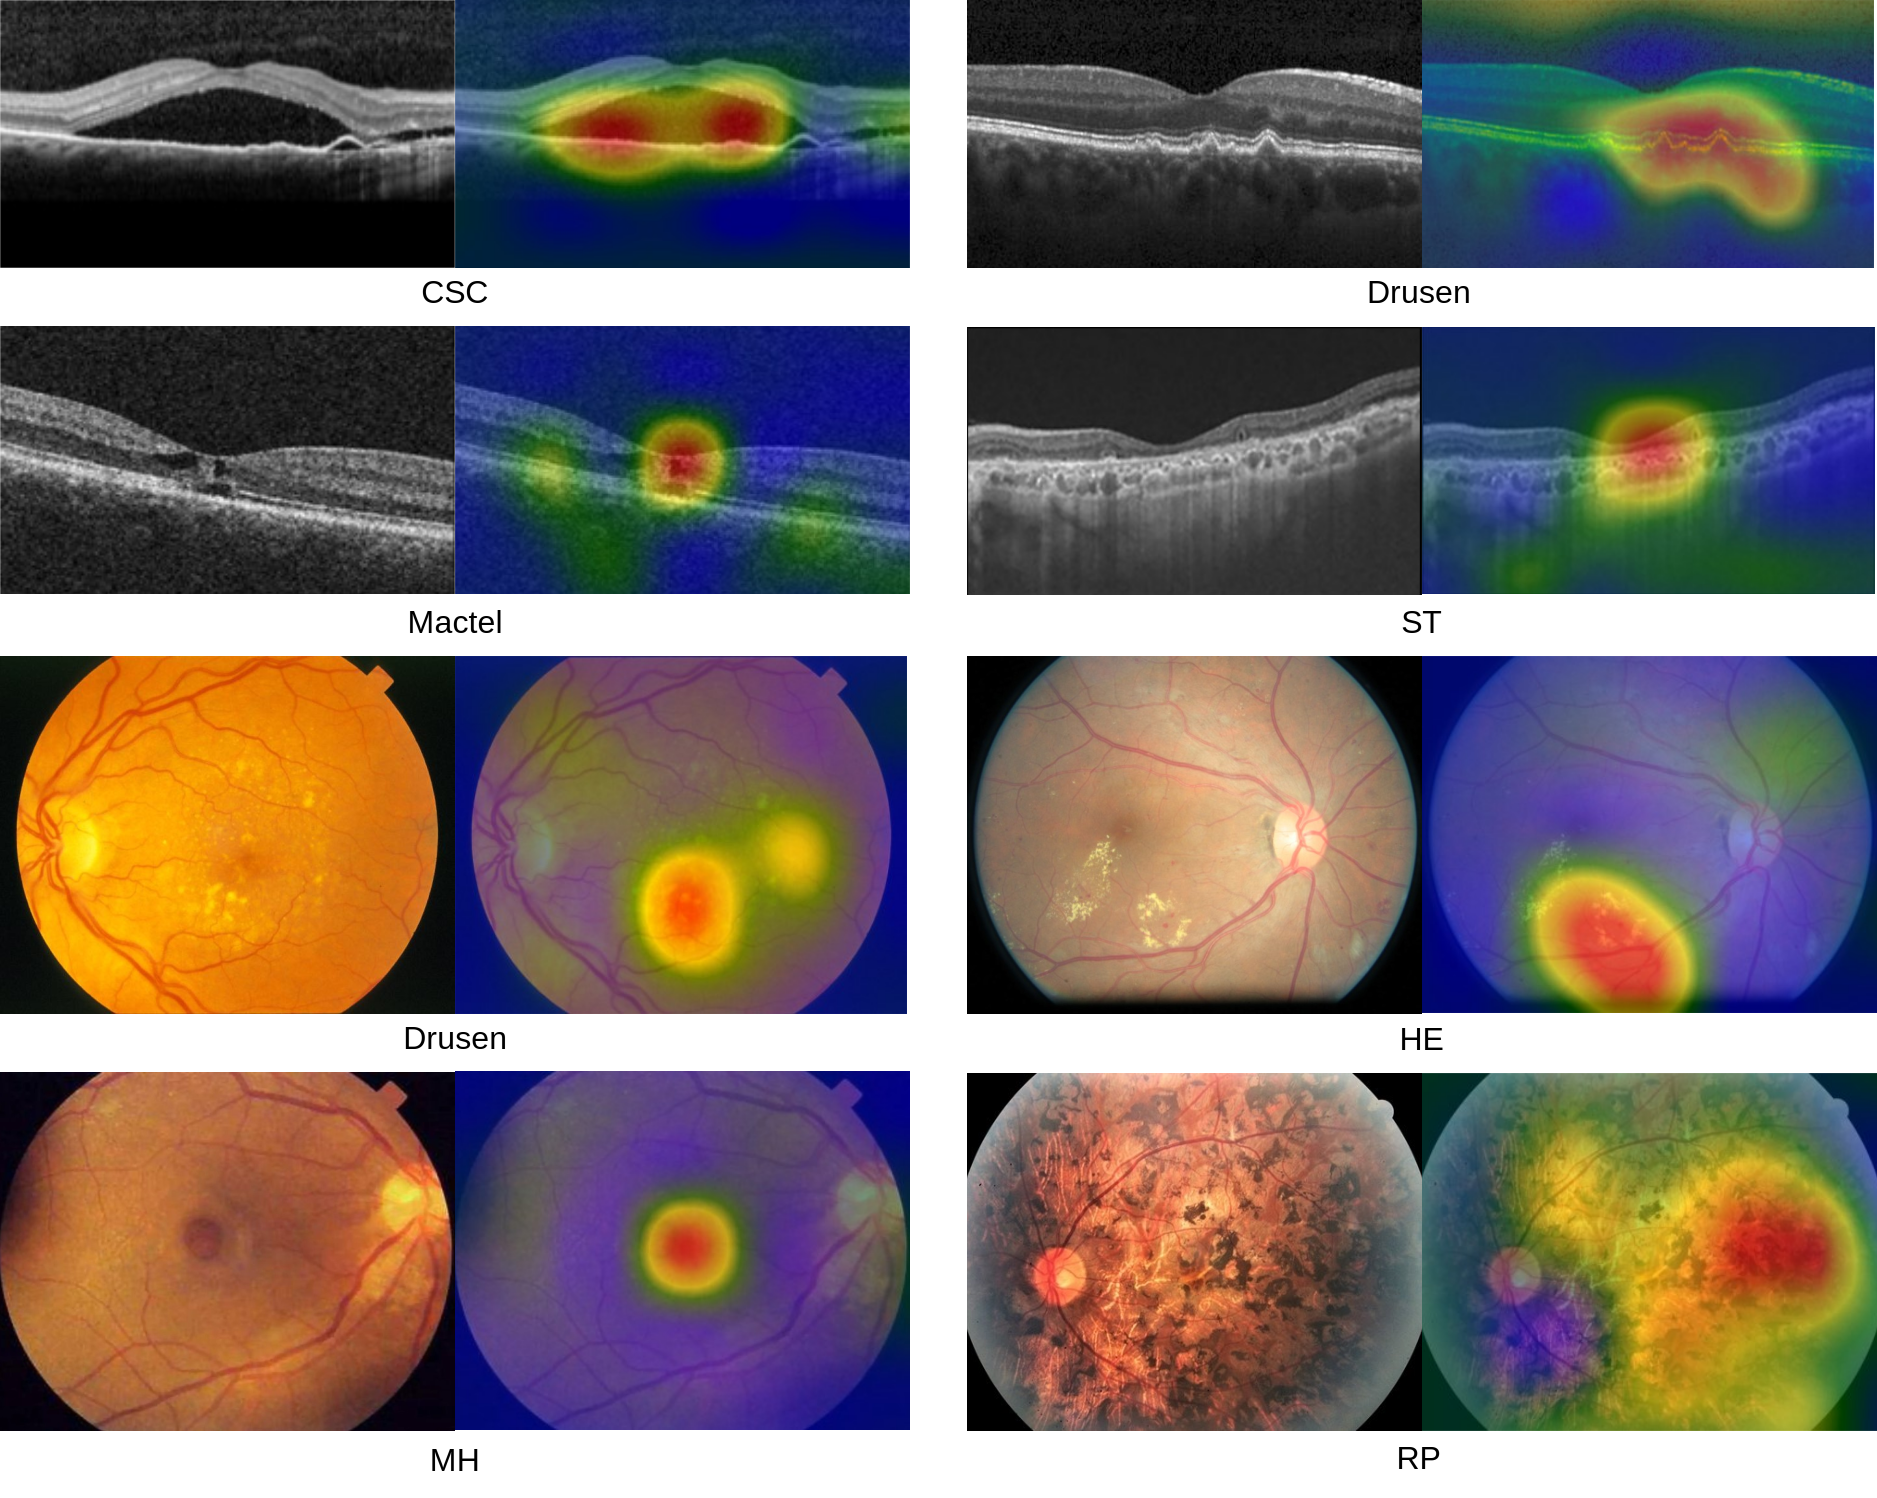
\includegraphics[width=\linewidth]{Figs/abnormity_gradCAM.png}
		\caption{GradCAM}
		\vspace{0.3cm}
		\label{fig:gradCAM}
	\end{figure}
	\begin{figure}[htbp]
		\centering
		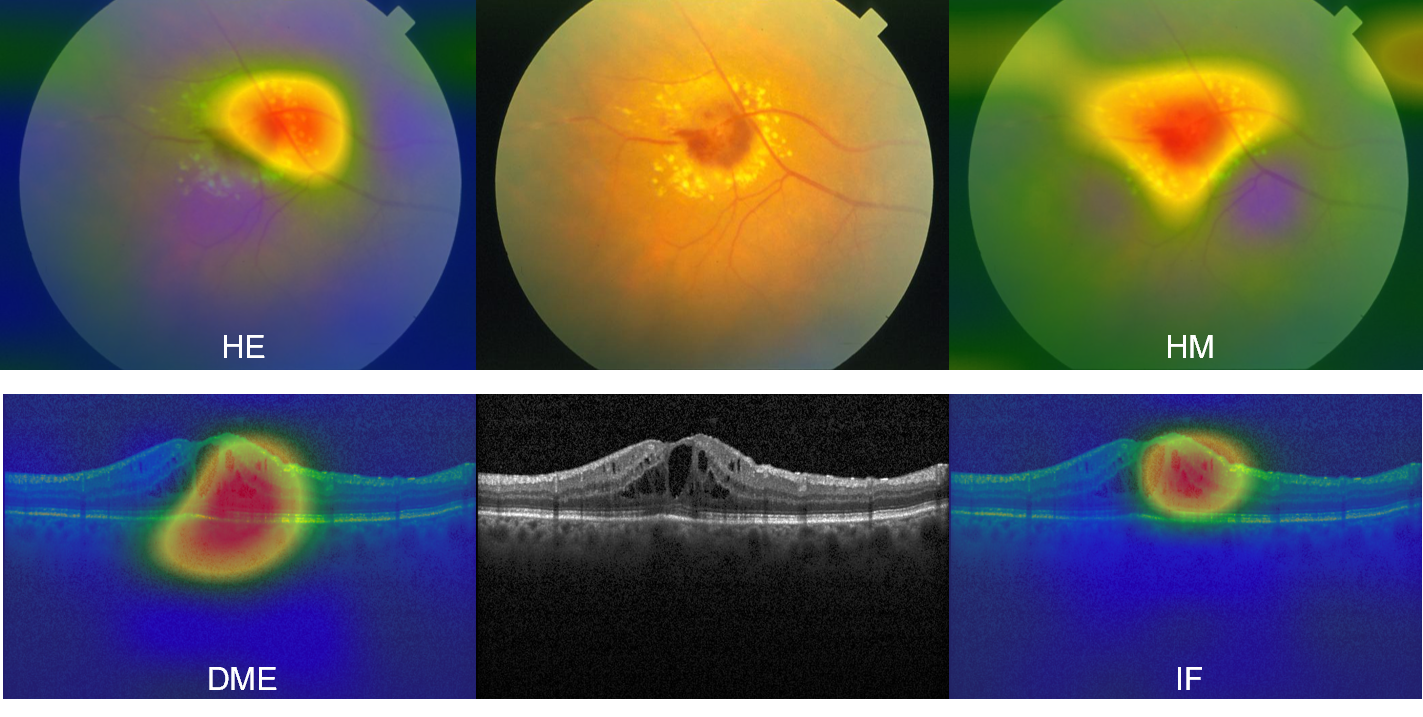
\includegraphics[width=0.8\linewidth]{Figs/abnormity_gradCAM_multiple_abnormities.png}
		\caption{GradCAM with multiple abnormities}
		\vspace{0.3cm}
		\label{fig:gradCAM_multi_abnormity}
	\end{figure}
	
	\section{Diagnosis Model}
	
	\subsection{Data Preparation}
	
	TEXT: how to choose data (with an example)
	how to find level (number of traits = level for the disease as label during training)
	
	
	\subsection{Training}
	
	TEXT: hyperparameters, software, hardware
	
	TEXT: comments
	
	
	\subsection{Results}
	
	TEXT: D1 output - calculate expected grade. in order to compare, divide by total number of traits for this disease so that normalized grade falls in [0, 1]. 
	used for checking number of abnormities associated to the disease
	
	TEXT: top-probs method
	
	\begin{table}[htbp]
		\centering
		\caption{Diagnosis Test}
		\label{tb:diagnosis_test}
		\pgfplotstabletypeset[
		multicolumn names,
		col sep=comma,
		columns = {Abnormity, Precision, Sensitivity, Specificity, FOne, AUC},
		columns/Abnormity/.style={string type, column name=Abnormities},
		columns/Precision/.style={string type, column name=Precision},
		columns/Sensitivity/.style={string type, column name=Sensitivity},
		columns/Specificity/.style={string type, column name=Specificity},
		columns/FOne/.style={string type, column name={F1 Score}},
		columns/AUC/.style={string type, column name=AUC},
		every head row/.style={before row=\toprule, after row=\midrule},
		every last row/.style={ after row=\bottomrule}
		]{Tables/diagnosis2.csv}
	\end{table}
	
	\begin{figure}[htbp]
		\centering
		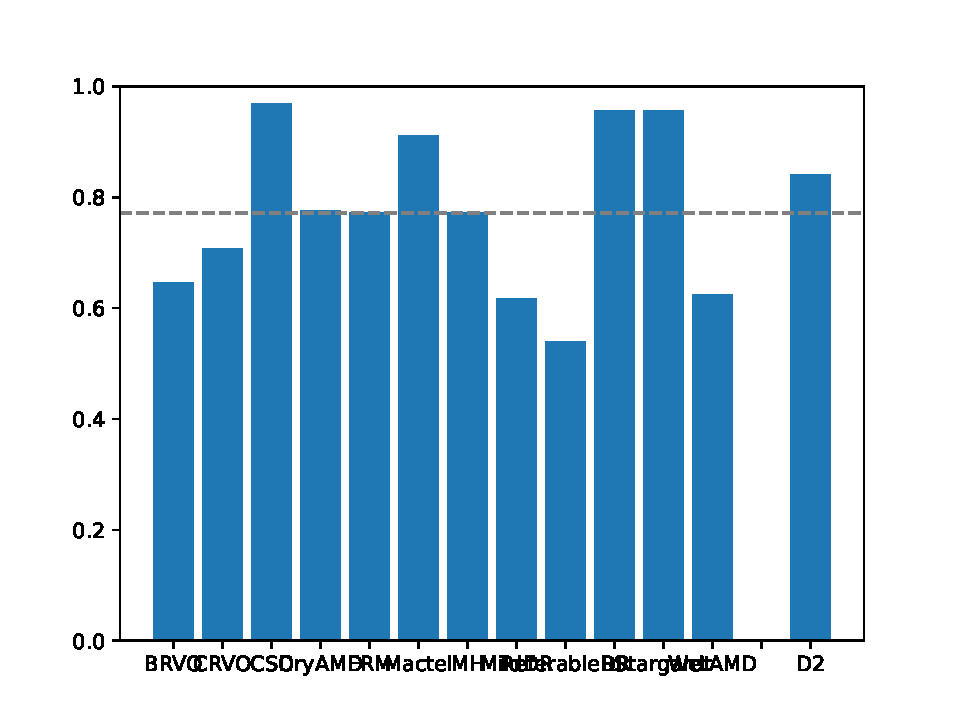
\includegraphics[width=\linewidth]{Figs/diagnosis1_acc_barchart.pdf}
		\caption{D1 Acc Bar}
		\vspace{0.3cm}
		\label{fig:D1_acc_bar}
	\end{figure}
	
	\begin{figure}[htbp]
		\centering
		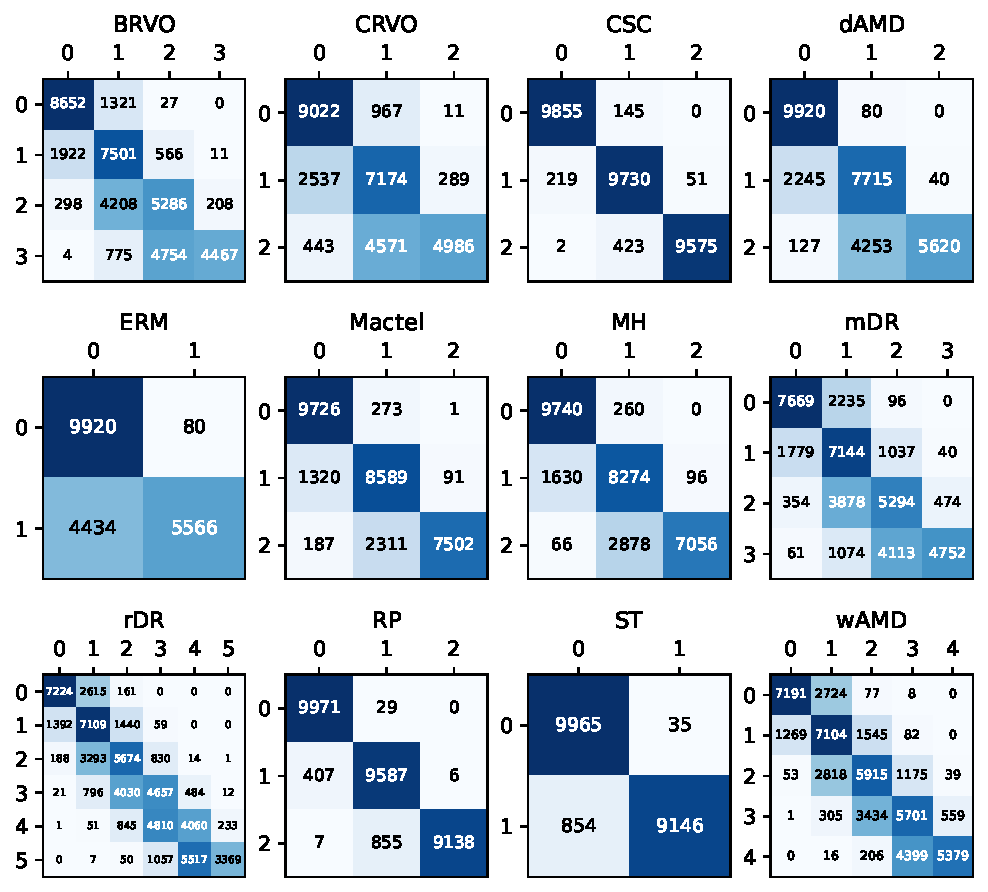
\includegraphics[width=\linewidth]{Figs/diagnosis1_confusion_matrix.pdf}
		\caption{D1 Conf Mat}
		\vspace{0.3cm}
		\label{fig:D1_conf_mat}
	\end{figure}
	TEXT: comments
	
	\begin{figure}[htbp]
		\centering
		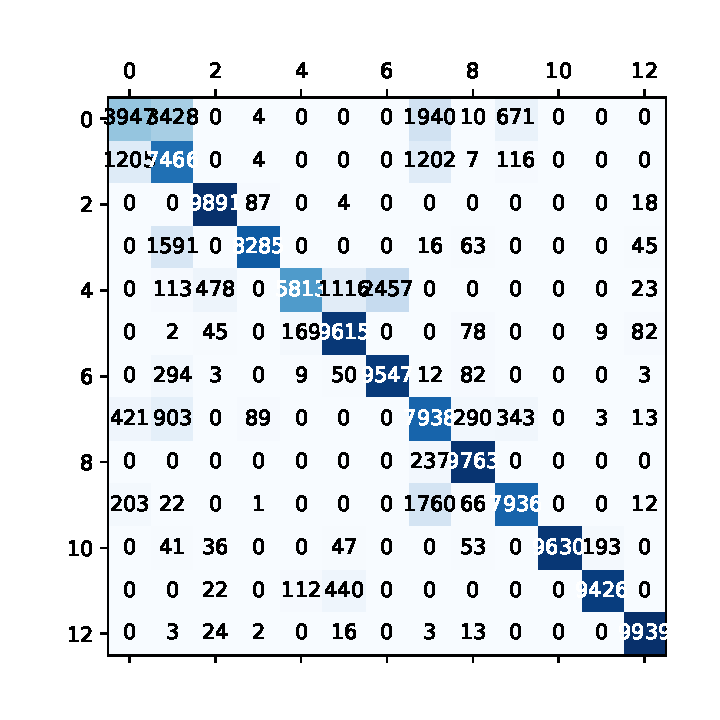
\includegraphics[width=\linewidth]{Figs/diagnosis2_confusion_matrix.pdf}
		\caption{D2 Conf Mat}
		\vspace{0.3cm}
		\label{fig:D2_conf_mat}
	\end{figure}
	\begin{figure}[htbp]
		\centering
		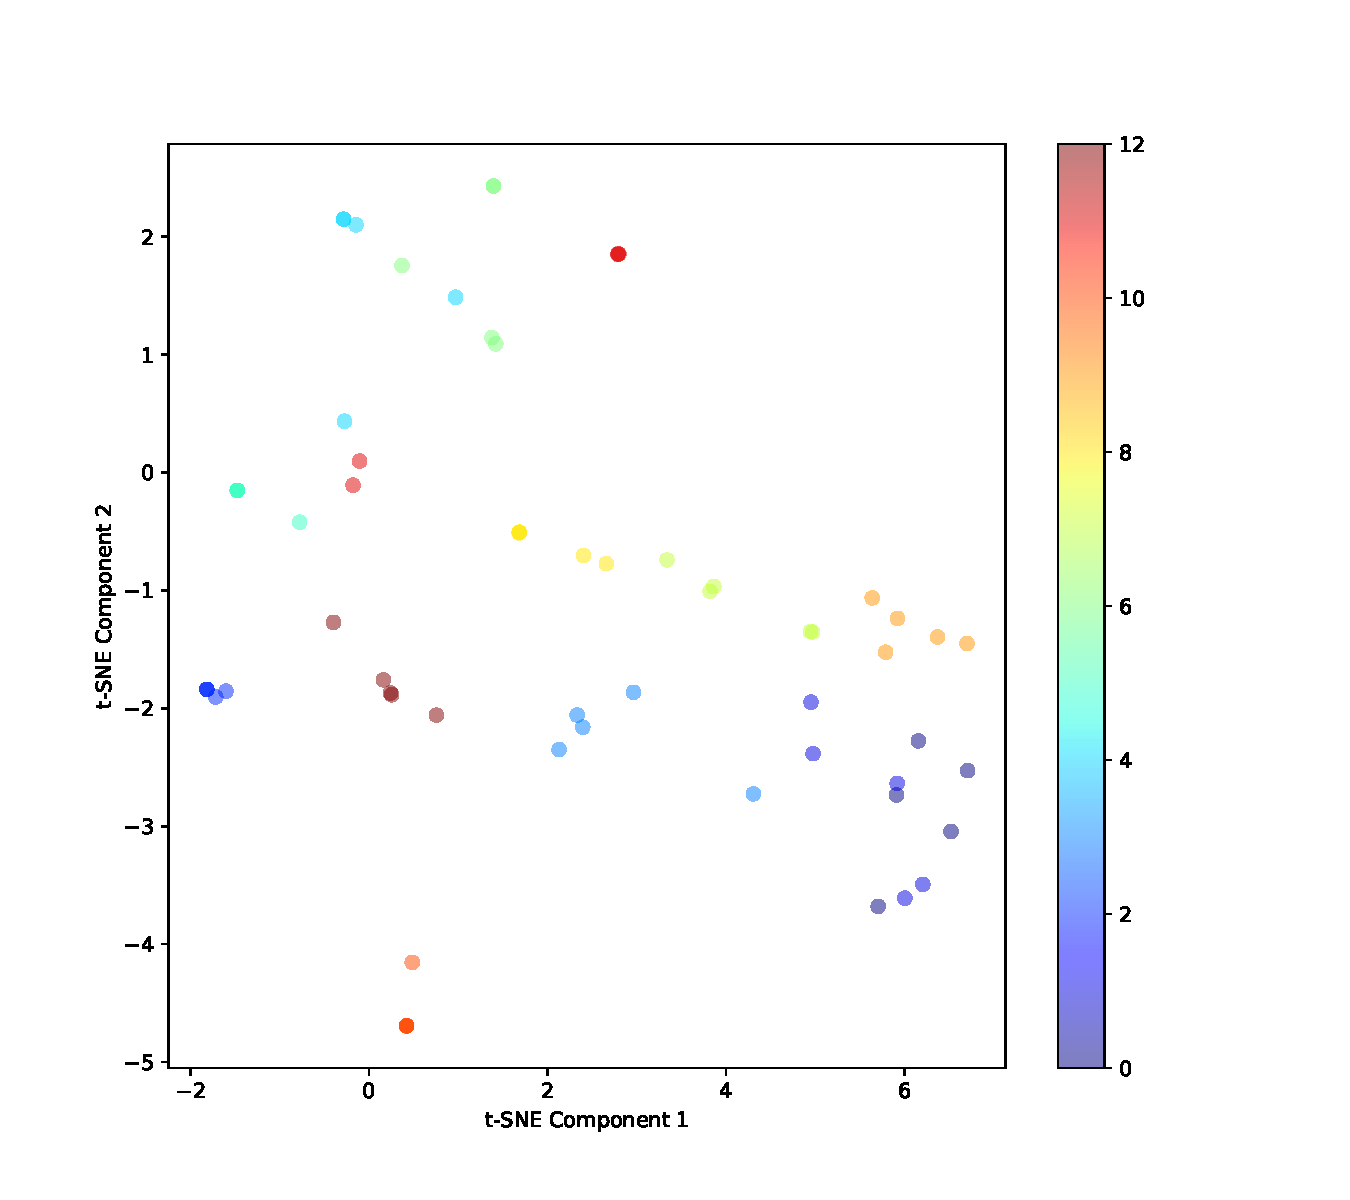
\includegraphics[width=\linewidth]{Figs/diagnosis2_tSNE.pdf}
		\caption{D2 tSNE}
		\vspace{0.3cm}
		\label{fig:D2_tSNE}
	\end{figure}
	TEXT: comments
	
	\begin{figure}[htbp]
		\centering
		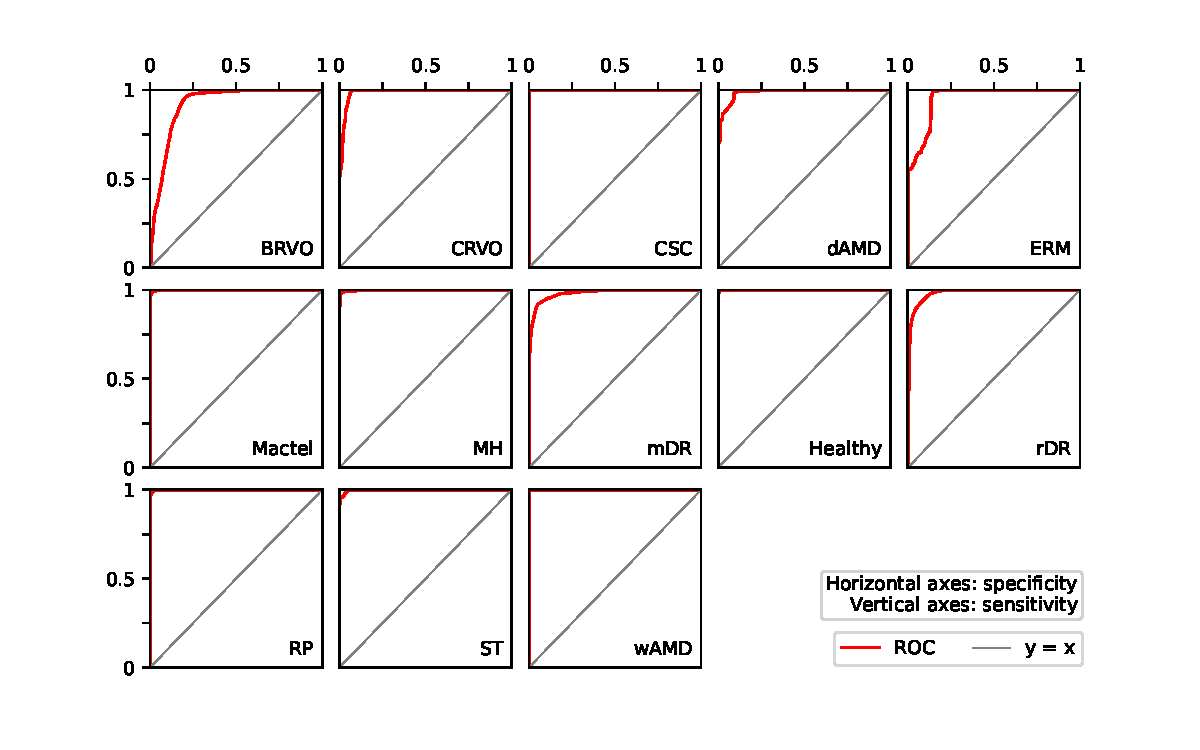
\includegraphics[width=\linewidth]{Figs/diagnosis2_ROC.pdf}
		\caption{D2 ROC}
		\vspace{0.3cm}
		\label{fig:D2_ROC}
	\end{figure}
	TEXT: comparison and comments
	
	\section{Discussion}
	
	TEXT: Do two models increase accuracy? How?
	
	TEXT: Comparison to other studies
	
	TEXT: Strengths and weaknesses
	how to improve
	
	\section{Conclusion}
	
	TEXT: conclusion
	
	\phantomsection
	\addcontentsline{toc}{section}{References}
	\newrefcontext[sorting=nyt]
	\printbibliography
	
	\pagebreak
	\section*{Appendix}
	
	List: Google Image source links
	
	Table: abnormities with description (edit the two tables below; ALPHABETICAL ORDER!!!)
	
	{
		\fontsize{9}{12}\selectfont
		{
			\begin{longtable}{lp{3.8in}}
				\caption{OCT Abnormities}
				\label{tb:oct-abnormites}\\
				\toprule
				Abnormity&Description\\
				\toprule
				
				\multicolumn{1}{l}{Central serous chorioretinopathy (CSC)}
				& \multicolumn{1}{l}{The accumulation of fluid underneath the retina.}\\
				
				\multicolumn{1}{l}{Epiretinal membrane (ERM)}
				& A thin layer of fibrous tissue forms on the surface of the retina, particularly the macula.\\
				
				\multicolumn{1}{l}{Macular hole (MH)}
				& Disruption or discontinuity in the normal retinal layers surrounding the macular hole.\\
				
				\multicolumn{1}{l}{Stargardt disease}
				& Thinning and atrophy of the retina. Disruption of photoreceptor layers. Presence of subretinal deposits.\\
				
				\multicolumn{1}{l}{Retinitis pigmentosa (RP)}
				& Thinning of the Retinal Layers. Disruption of Photoreceptor Layers. Attenuation of Retinal Vasculature.\\
				
				\multicolumn{1}{l}{Macular telangiectasia (Mactel)}
				& Abnormalities in the macular blood vessels, leading to changes in the macular structure and function\\
				
				\multicolumn{1}{l}{Diabetic macular edema (DME)}
				& The accumulation of fluid in the macula. \\
				
				\multicolumn{1}{l}{Choroidal neovascularization}
				& The abnormal growth of new blood vessels in the choroid layer.\\
				
				\multicolumn{1}{l}{Subretinal fluid}
				& The accumulation of fluid between the neurosensory retina and the retinal pigment epithelium (RPE)\\
				
				\multicolumn{1}{l}{Intraretinal fluid}
				& The accumulation of fluid within the layers of the retina.\\
				
				\multicolumn{1}{l}{Drusen}
				& Small deposits of extracellular material that accumulate beneath the retinal pigment epithelium (RPE) or between the RPE and the photoreceptor layer in the macular region of the retina.\\
				
				\bottomrule
			\end{longtable}
		}
	}
	
	{
		\fontsize{9}{12}\selectfont
		{
			\begin{longtable}{lp{3.8in}}
				\caption{Fundus Abnormalities}
				\label{tb:fundus-ab}\\
				\toprule
				Abnormity&Description\\
				\toprule
				
				\multicolumn{1}{l}{Retinitis pigmentosa (RP)}
				& Description of RP\\
				
				\multicolumn{1}{l}{Microaneurysm}
				& Description of microaneurysm\\
				
				\multicolumn{1}{l}{Macular hole (MH)} & Full-thickness macular hole showing a surrounding cuff of subretinal fluid.\\
				
				\multicolumn{1}{l}{Hard exudate} & Yellow or Yellow-White Deposits. Hard Borders. Distribution. Clustering Around Blood Vessels\\
				
				\multicolumn{1}{l}{Hemorrhage} & Small dot-like to larger blot. Fresh hemorrhages typically appear bright red or deep red in color, indicating the presence of oxygenated blood. Over time, as the blood undergoes degradation and clotting, the hemorrhage may change color to darker red, orange, or yellowish hues.\\
				
				\multicolumn{1}{l}{Cotton wool patch / soft exudate} & White or off-white lesions. Irregular shapes and margins.\\
				
				\multicolumn{1}{l}{Vascular abnormity} & Retinal Vessel Tortuosity. Retinal Vessel Caliber Changes. \\
				
				\multicolumn{1}{l}{Drusen} & Small, round or oval-shaped yellow or white deposits.\\
				
				\bottomrule
			\end{longtable}
		}
	}
	
	
	\begin{figure}[htbp]
		\centering
		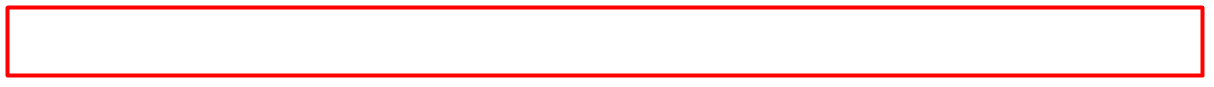
\includegraphics[width=\linewidth]{Figs/Temp.png}
		\caption{Result Page}
		\vspace{0.3cm}
		\label{fig:result_page}
	\end{figure}
	
	TEXT: APP/website description
	
	Link: GitHub repo
	
\end{document}